\documentclass[aspectratio=169,10pt]{beamer}

\usetheme{Madrid}
\usecolortheme{default}

\usepackage[T1]{fontenc}
\usepackage[utf8]{inputenc}
\usepackage{lmodern}
\usepackage{booktabs}
\usepackage{tabularx}
\usepackage{array}
\usepackage{tikz}
\usepackage{graphicx}
\usepackage{amsmath}
\usetikzlibrary{positioning,arrows.meta}

\definecolor{epflred}{RGB}{220,0,0}
\definecolor{soxblue}{RGB}{24,55,91}
\definecolor{softgray}{RGB}{245,247,250}
\definecolor{darkgray}{RGB}{55,65,81}
\definecolor{goodgreen}{RGB}{18,128,92}
\definecolor{warmorange}{RGB}{207,112,31}

\setbeamercolor{structure}{fg=epflred}
\setbeamercolor{frametitle}{fg=white,bg=soxblue}
\setbeamercolor{title}{fg=white,bg=soxblue}
\setbeamercolor{block title}{fg=white,bg=soxblue}
\setbeamercolor{block body}{fg=black,bg=softgray}
\setbeamercolor{alerted text}{fg=epflred}
\setbeamertemplate{navigation symbols}{}
\setbeamertemplate{footline}[frame number]

\newcommand{\sox}{SOX}
\newcommand{\simsox}{simSOX}
\newcommand{\gas}[1]{\textbf{#1 gas}}
\newcommand{\giB}{GiB}
\newcommand{\kib}{KiB}

\title[Gas-Aware SOX]{Gas-Aware Implementation of Sponsored Fair Exchange}
\subtitle{Semester Project at LASEC}
\author[Ryad Mohamed Aouak]{Ryad Mohamed Aouak}
\institute[EPFL LASEC]{Supervisor: Prof. Serge Vaudenay\\EPFL, LASEC}
\date{Semester Project Presentation}

\begin{document}

\begin{frame}
  \titlepage
  \vspace{-1em}
  \begin{center}
    
\includegraphics[height=0.65cm]{../report/figures/logo_epfl_coul.pdf}
    \hspace{1.5em}
    
\includegraphics[height=0.65cm]{../report/figures/logo_lasec_coul.pdf}
  \end{center}
\end{frame}

\begin{frame}{A simple question}
  \begin{center}
    \Large
    How can Alice buy a digital file from Bob\\
    \vspace{0.4em}
    \textbf{without either side having to trust the other?}
  \end{center}
  \vspace{1.0em}
  \begin{columns}[T,onlytextwidth]
    \begin{column}{0.48\textwidth}
      \begin{block}{If Bob sends first}
        Alice may keep the file and never pay.
      \end{block}
    \end{column}
    \begin{column}{0.48\textwidth}
      \begin{block}{If Alice pays first}
        Bob may keep the money and send nothing, or send a wrong file.
      \end{block}
    \end{column}
  \end{columns}
  \vfill
  \centering
  \textit{This is the fair-exchange problem.}
\end{frame}

\begin{frame}{Fair exchange target}
  \begin{columns}[T,onlytextwidth]
    \begin{column}{0.52\textwidth}
      \begin{block}{Desired outcome}
        Either both parties get what they should, or the exchange is cancelled.
      \end{block}
      \begin{itemize}
        \item The buyer receives an item matching a public description.
        \item The vendor receives the payment.
        \item No trusted human judge checks every file.
      \end{itemize}
    \end{column}
    \begin{column}{0.44\textwidth}
      \centering
      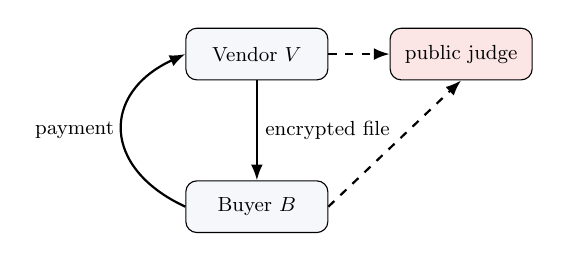
\begin{tikzpicture}[scale=0.82,transform shape, node distance=0.95cm, every node/.style={font=\small}]
        \node[draw,rounded corners,fill=softgray,minimum width=2.2cm,minimum height=0.8cm] (v) {Vendor \(V\)};
        \node[draw,rounded corners,fill=softgray,minimum width=2.2cm,minimum height=0.8cm,below=1.55cm of v] (b) {Buyer \(B\)};
        \node[draw,rounded corners,fill=epflred!10,minimum width=2.2cm,minimum height=0.8cm,right=0.95cm of v] (j) {public judge};
        \draw[-{Latex[length=2mm]},thick] (v) -- node[right]{encrypted file} (b);
        \draw[-{Latex[length=2mm]},thick] (b.west) .. controls +(-1.3,0.6) and +(-1.3,-0.6) .. node[left]{payment} (v.west);
        \draw[-{Latex[length=2mm]},dashed,thick] (v.east) -- (j.west);
        \draw[-{Latex[length=2mm]},dashed,thick] (b.east) -- (j.south);
      \end{tikzpicture}
    \end{column}
  \end{columns}
\end{frame}

\begin{frame}{Why a smart contract appears}
  \begin{block}{Mental model for this talk}
    A smart contract is a public, deterministic judge that can hold deposits and enforce payouts.
  \end{block}
  \vspace{0.8em}
  \begin{columns}[T,onlytextwidth]
    \begin{column}{0.48\textwidth}
      \begin{block}{Good news}
        It can replace an always-online trusted third party.
      \end{block}
    \end{column}
    \begin{column}{0.48\textwidth}
      \begin{block}{Bad news}
        Every public computation and every deployment costs \textbf{gas}.
      \end{block}
    \end{column}
  \end{columns}
  \vfill
  \begin{center}
    \Large \alert{So the real engineering question is: what must be public, and what can stay local?}
  \end{center}
\end{frame}

\begin{frame}{The SOX idea in one picture}
  \begin{center}
    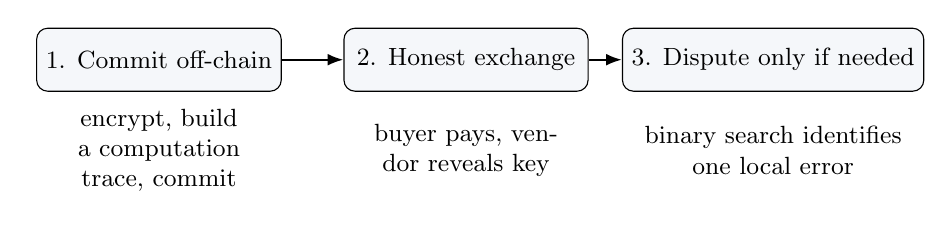
\begin{tikzpicture}[x=1cm,y=1cm, every node/.style={font=\small}]
      \node[draw,rounded corners,fill=softgray,minimum width=3.1cm,minimum height=0.8cm] at (0,0) (p) {1. Commit off-chain};
      \node[draw,rounded corners,fill=softgray,minimum width=3.1cm,minimum height=0.8cm] at (3.9,0) (h) {2. Honest exchange};
      \node[draw,rounded corners,fill=softgray,minimum width=3.1cm,minimum height=0.8cm] at (7.8,0) (d) {3. Dispute only if needed};
      \draw[-{Latex[length=2mm]},thick] (p) -- (h);
      \draw[-{Latex[length=2mm]},thick] (h) -- (d);
      \node[align=center,text width=3.1cm] at (0,-1.15) {encrypt, build a computation trace, commit};
      \node[align=center,text width=3.1cm] at (3.9,-1.15) {buyer pays, vendor reveals key};
      \node[align=center,text width=3.3cm] at (7.8,-1.15) {binary search identifies one local error};
    \end{tikzpicture}
  \end{center}
  \vspace{0.8em}
  \begin{block}{Optimistic protocol}
    If everyone behaves honestly, the expensive verification never happens on-chain.
  \end{block}
\end{frame}

\begin{frame}{The cryptographic object behind SOX}
  \begin{columns}[T,onlytextwidth]
    \begin{column}{0.47\textwidth}
      \begin{block}{Off-chain}
        The implementation builds a compact circuit/trace for:
        \begin{itemize}
          \item AES-CTR decryption;
          \item SHA-256 description check;
          \item commitments to ciphertext, circuit, and intermediate values.
        \end{itemize}
      \end{block}
    \end{column}
    \begin{column}{0.49\textwidth}
      \begin{block}{On-chain}
        The contract stores short commitments and later verifies:
        \begin{itemize}
          \item membership proofs;
          \item one local gate computation;
          \item the final payout decision.
        \end{itemize}
      \end{block}
    \end{column}
  \end{columns}
  \vfill
  \centering
  \textit{The file can be huge; the public judge should only see small authenticated pieces.}
\end{frame}

\begin{frame}{Baseline SOX flow}
  \begin{columns}[T,onlytextwidth]
    \begin{column}{0.48\textwidth}
      \begin{block}{Optimistic path}
        \begin{enumerate}
          \item \(V\) commits to the encrypted exchange data.
          \item \(S\) funds the optimistic contract.
          \item \(B\) pays.
          \item \(V\) reveals the key.
          \item If \(B\) accepts, \(V\) is paid.
        \end{enumerate}
      \end{block}
    \end{column}
    \begin{column}{0.48\textwidth}
      \begin{block}{Dispute path}
        \begin{enumerate}
          \item \(B\) complains.
          \item \(S_B\) and \(S_V\) fund the dispute.
          \item A binary search narrows the disagreement.
          \item One local step is verified on-chain.
          \item The contract finalizes payouts.
        \end{enumerate}
      \end{block}
    \end{column}
  \end{columns}
  \vspace{0.5em}
  \centering
  \textit{My work keeps this goal but changes how it is implemented and measured.}
\end{frame}

\begin{frame}{What I inherited}
  \begin{columns}[T,onlytextwidth]
    \begin{column}{0.48\textwidth}
      \begin{block}{Already working}
        \begin{itemize}
          \item Rust/WebAssembly precontract pipeline.
          \item Solidity optimistic and dispute contracts.
          \item Local web application and backend.
          \item Sponsored transaction infrastructure.
        \end{itemize}
      \end{block}
    \end{column}
    \begin{column}{0.48\textwidth}
      \begin{block}{Main problems}
        \begin{itemize}
          \item Expensive per-exchange deployments.
          \item No clean implementation of the main variants.
          \item Gas numbers were hard to compare.
          \item Browser path not suitable for 1 \giB{} benchmarks.
        \end{itemize}
      \end{block}
    \end{column}
  \end{columns}
\end{frame}

\begin{frame}{My project roadmap}
  \begin{center}
    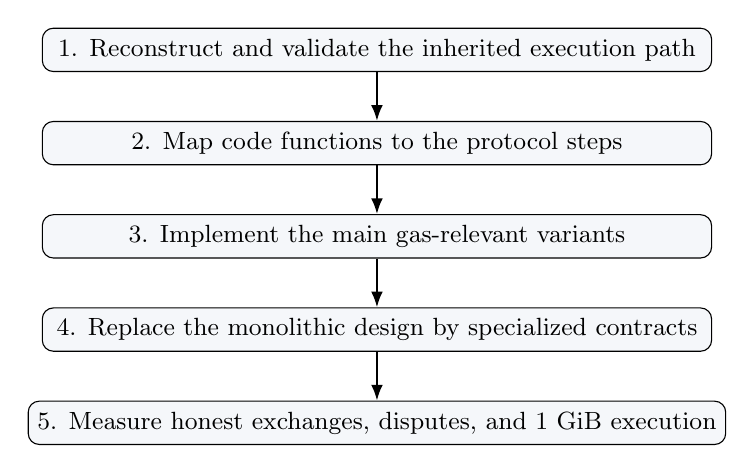
\begin{tikzpicture}[node distance=0.62cm, every node/.style={font=\small}]
      \node[draw,rounded corners,fill=softgray,minimum width=8.5cm,minimum height=0.55cm] (a) {1. Reconstruct and validate the inherited execution path};
      \node[draw,rounded corners,fill=softgray,minimum width=8.5cm,minimum height=0.55cm,below=of a] (b) {2. Map code functions to the protocol steps};
      \node[draw,rounded corners,fill=softgray,minimum width=8.5cm,minimum height=0.55cm,below=of b] (c) {3. Implement the main gas-relevant variants};
      \node[draw,rounded corners,fill=softgray,minimum width=8.5cm,minimum height=0.55cm,below=of c] (d) {4. Replace the monolithic design by specialized contracts};
      \node[draw,rounded corners,fill=softgray,minimum width=8.5cm,minimum height=0.55cm,below=of d] (e) {5. Measure honest exchanges, disputes, and 1 \giB{} execution};
      \draw[-{Latex[length=2mm]},thick] (a) -- (b);
      \draw[-{Latex[length=2mm]},thick] (b) -- (c);
      \draw[-{Latex[length=2mm]},thick] (c) -- (d);
      \draw[-{Latex[length=2mm]},thick] (d) -- (e);
    \end{tikzpicture}
  \end{center}
\end{frame}

\begin{frame}{The variants: who pays and when?}
  \begin{columns}[T,onlytextwidth]
    \begin{column}{0.31\textwidth}
      \begin{block}{Before exchange}
        \begin{itemize}
          \item normal SOX;
          \item \simsox{} / no \(S\)-deposit;
          \item \(S=B\);
          \item \(S=V\).
        \end{itemize}
      \end{block}
    \end{column}
    \begin{column}{0.31\textwidth}
      \begin{block}{During dispute}
        \begin{itemize}
          \item \(S_B=B\);
          \item \(S_V=V\);
          \item fewer repeated challenge loops.
        \end{itemize}
      \end{block}
    \end{column}
    \begin{column}{0.31\textwidth}
      \begin{block}{For SHA-256 descriptions}
        \begin{itemize}
          \item circuit is determined by \(|x|\);
          \item no generic \(\pi_1\) proof;
          \item contract reconstructs the gate.
        \end{itemize}
      \end{block}
    \end{column}
  \end{columns}
\end{frame}

\begin{frame}{A useful negative result}
  \begin{columns}[T,onlytextwidth]
    \begin{column}{0.50\textwidth}
      \begin{block}{First implementation attempt}
        Put all variants into the same large contracts.
      \end{block}
      \begin{itemize}
        \item Easy to validate.
        \item Bad for gas.
        \item Every user pays for branches they do not use.
      \end{itemize}
    \end{column}
    \begin{column}{0.46\textwidth}
      \begin{center}
        \begin{tabular}{lrr}
          \toprule
          Honest path & Initial & Monolithic \\
          \midrule
          Deployment & 2.08M & 2.81M \\
          Execution & 0.22M & 0.23M \\
          \midrule
          Total & 2.30M & 3.05M \\
          \bottomrule
        \end{tabular}
      \end{center}
      \vspace{0.5em}
      \centering
      \alert{+32.46\% gas}
    \end{column}
  \end{columns}
  \vfill
  \centering
  \Large \textbf{This forced the architectural pivot.}
\end{frame}

\begin{frame}{Final architecture}
  \begin{center}
    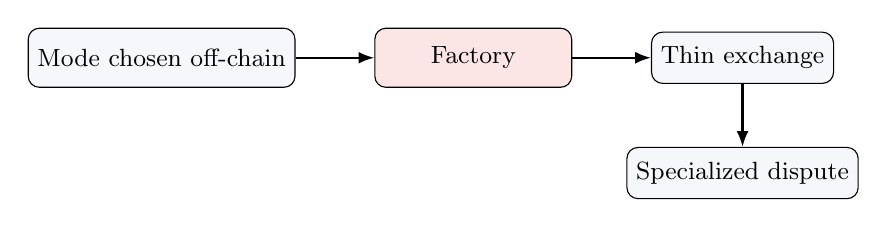
\begin{tikzpicture}[node distance=0.95cm, every node/.style={font=\small}]
      \node[draw,rounded corners,fill=softgray,minimum width=3.1cm,minimum height=0.75cm] (choice) {Mode chosen off-chain};
      \node[draw,rounded corners,fill=epflred!10,minimum width=2.5cm,minimum height=0.75cm,right=1.0cm of choice] (factory) {Factory};
      \node[draw,rounded corners,fill=softgray,minimum width=2.2cm,minimum height=0.65cm,right=1.0cm of factory] (clone) {Thin exchange};
      \node[draw,rounded corners,fill=softgray,minimum width=2.2cm,minimum height=0.65cm,below=0.8cm of clone] (dispute) {Specialized dispute};
      \draw[-{Latex[length=2mm]},thick] (choice) -- (factory);
      \draw[-{Latex[length=2mm]},thick] (factory) -- (clone);
      \draw[-{Latex[length=2mm]},thick] (clone) -- (dispute);
    \end{tikzpicture}
  \end{center}
  \vspace{0.8em}
  \begin{block}{Design principle}
    If a mode is known before execution, do not deploy code for the other modes.
  \end{block}
  \begin{block}{Practical effect}
    Reusable code is deployed once; each exchange pays only for a small specialized instance.
  \end{block}
\end{frame}

\begin{frame}{What I implemented}
  \small
  \begin{tabularx}{\linewidth}{>{\raggedright\arraybackslash}p{0.26\linewidth}>{\raggedright\arraybackslash}X}
    \toprule
    Area & Contribution \\
    \midrule
    Solidity contracts &
    Specialized optimistic clones, \texttt{SOXFactory}, self-sponsored dispute contracts,
    hardcoded SHA-256 dispute verifier. \\
    Rust/native tooling &
    Native large-file precontract and hardcoded dispute witness generation. \\
    Frontend/backend &
    User-facing mode selection and storage of the selected precontract variant. \\
    Tests and measurements &
    Same-scope gas benchmarks, 16 \kib{} dispute variants, complete 1 \giB{} hardcoded benchmark. \\
    Report methodology &
    Clear separation between one-time, marginal, dispute, and local runtime costs. \\
    \bottomrule
  \end{tabularx}
\end{frame}

\begin{frame}{Result 1: honest exchange cost}
  \begin{columns}[T,onlytextwidth]
    \begin{column}{0.44\textwidth}
      \begin{block}{Initial implementation}
        Full optimistic account per exchange:
        \[
          \gas{2,300,201}
        \]
      \end{block}
      \begin{block}{One-time setup}
        Factory + implementations:
        \[
          \gas{6,584,001}
        \]
      \end{block}
    \end{column}
    \begin{column}{0.52\textwidth}
      \begin{center}
        \begin{tabular}{lrr}
          \toprule
          Final mode & Per exchange & Gain \\
          \midrule
          \simsox{} & 500,720 & -78.23\% \\
          \(S=B\) & 516,349 & -77.55\% \\
          \(S=V\) & 556,309 & -75.81\% \\
          \bottomrule
        \end{tabular}
      \end{center}
      \vspace{0.8em}
      \centering
      \Large \textcolor{goodgreen}{about 4x cheaper per new exchange}
    \end{column}
  \end{columns}
\end{frame}

\begin{frame}{Result 2a: the baseline comparison window}
  \begin{center}
    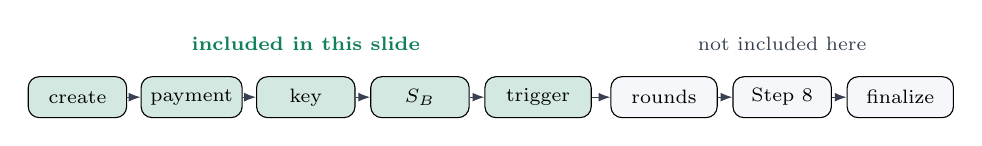
\begin{tikzpicture}[x=1cm,y=1cm, every node/.style={font=\scriptsize}]
      \node[draw, rounded corners, fill=goodgreen!18, minimum width=1.25cm, minimum height=0.52cm] (create) at (0,0) {create};
      \node[draw, rounded corners, fill=goodgreen!18, minimum width=1.25cm, minimum height=0.52cm] (pay) at (1.45,0) {payment};
      \node[draw, rounded corners, fill=goodgreen!18, minimum width=1.25cm, minimum height=0.52cm] (key) at (2.9,0) {key};
      \node[draw, rounded corners, fill=goodgreen!18, minimum width=1.25cm, minimum height=0.52cm] (sb) at (4.35,0) {\(S_B\)};
      \node[draw, rounded corners, fill=goodgreen!18, minimum width=1.35cm, minimum height=0.52cm] (trigger) at (5.85,0) {trigger};
      \node[draw, rounded corners, fill=softgray, minimum width=1.35cm, minimum height=0.52cm] (rounds) at (7.45,0) {rounds};
      \node[draw, rounded corners, fill=softgray, minimum width=1.25cm, minimum height=0.52cm] (step8) at (8.95,0) {Step 8};
      \node[draw, rounded corners, fill=softgray, minimum width=1.35cm, minimum height=0.52cm] (final) at (10.45,0) {finalize};
      \foreach \a/\b in {create/pay,pay/key,key/sb,sb/trigger,trigger/rounds,rounds/step8,step8/final}
        \draw[-{Latex[length=1.5mm]}, darkgray] (\a) -- (\b);
      \node[goodgreen, font=\bfseries\scriptsize] at (2.9,0.68) {included in this slide};
      \node[darkgray, font=\scriptsize] at (8.95,0.68) {not included here};
    \end{tikzpicture}
  \end{center}

  \vspace{0.4em}
  \begin{center}
    \small
    \begin{tabularx}{\linewidth}{>{\raggedright\arraybackslash}Xr>{\raggedright\arraybackslash}X}
      \toprule
      Architecture & Gas & What changed? \\
      \midrule
      Initial implementation & 7,054,365 & baseline contract-per-exchange design \\
      Monolithic validator & 8,872,096 & all variants packed into one large contract \\
      Final normal clone & \textcolor{goodgreen}{5,495,184} & same normal protocol, cheaper clone architecture \\
      \bottomrule
    \end{tabularx}
  \end{center}

  \vspace{0.5em}
  \begin{block}{Takeaway}
    Same validated 4 MiB window in all architectures:
    \textcolor{goodgreen}{\(-22.10\%\) vs initial}. I stop here because the inherited
    implementation has no equally validated full-dispute baseline in the new variant scopes.
  \end{block}
\end{frame}

\begin{frame}{Result 2b: resolving the dispute segment}
  \begin{center}
    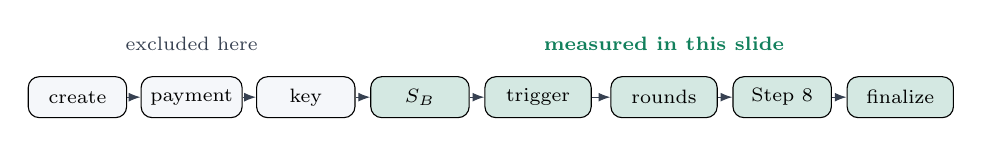
\begin{tikzpicture}[x=1cm,y=1cm, every node/.style={font=\scriptsize}]
      \node[draw, rounded corners, fill=softgray, minimum width=1.25cm, minimum height=0.52cm] (create) at (0,0) {create};
      \node[draw, rounded corners, fill=softgray, minimum width=1.25cm, minimum height=0.52cm] (pay) at (1.45,0) {payment};
      \node[draw, rounded corners, fill=softgray, minimum width=1.25cm, minimum height=0.52cm] (key) at (2.9,0) {key};
      \node[draw, rounded corners, fill=goodgreen!18, minimum width=1.25cm, minimum height=0.52cm] (sb) at (4.35,0) {\(S_B\)};
      \node[draw, rounded corners, fill=goodgreen!18, minimum width=1.35cm, minimum height=0.52cm] (trigger) at (5.85,0) {trigger};
      \node[draw, rounded corners, fill=goodgreen!18, minimum width=1.35cm, minimum height=0.52cm] (rounds) at (7.45,0) {rounds};
      \node[draw, rounded corners, fill=goodgreen!18, minimum width=1.25cm, minimum height=0.52cm] (step8) at (8.95,0) {Step 8};
      \node[draw, rounded corners, fill=goodgreen!18, minimum width=1.35cm, minimum height=0.52cm] (final) at (10.45,0) {finalize};
      \foreach \a/\b in {create/pay,pay/key,key/sb,sb/trigger,trigger/rounds,rounds/step8,step8/final}
        \draw[-{Latex[length=1.5mm]}, darkgray] (\a) -- (\b);
      \node[darkgray, font=\scriptsize] at (1.45,0.68) {excluded here};
      \node[goodgreen, font=\bfseries\scriptsize] at (7.45,0.68) {measured in this slide};
    \end{tikzpicture}
  \end{center}

  \vspace{0.4em}
  \begin{center}
    \small
    \begin{tabular}{lrrr}
      \toprule
      16 \kib{} segment \(S_B \rightarrow\) End & Monolithic & Final specialized & Gain \\
      \midrule
      Normal, external sponsors & 8,345,424 & 7,432,647 & -10.94\% \\
      Self-sponsored & 7,165,928 & 5,946,445 & -17.02\% \\
      Hardcoded SHA-256 & 8,310,230 & 5,195,022 & -37.49\% \\
      Self-sponsored + hardcoded & 7,193,323 & \textcolor{goodgreen}{4,042,185} & -43.81\% \\
      \bottomrule
    \end{tabular}
  \end{center}

  \vspace{0.5em}
  \begin{block}{Takeaway}
    Different window from the previous slide: this isolates dispute resolution variants,
    so the baseline is the monolithic validator that implements the same variants.
  \end{block}
\end{frame}

\begin{frame}{Hardcoded SHA-256: the most cryptographic optimization}
  \begin{columns}[T,onlytextwidth]
    \begin{column}{0.50\textwidth}
      \begin{block}{Generic mode}
        In Step 8, \(V\) provides:
        \begin{itemize}
          \item a gate description;
          \item a proof \(\pi_1\) that this gate belongs to \(h_{\mathit{circuit}}\);
          \item witness values for local verification.
        \end{itemize}
      \end{block}
    \end{column}
    \begin{column}{0.46\textwidth}
      \begin{block}{Hardcoded \(desc=\mathrm{SHA256}(x)\)}
        The contract reconstructs the expected gate from public metadata:
        \begin{itemize}
          \item file length;
          \item description hash;
          \item AES-CTR IV;
          \item gate index.
        \end{itemize}
      \end{block}
    \end{column}
  \end{columns}
  \vfill
  \centering
  \Large \alert{The vendor no longer supplies \(\pi_1\) or authoritative gate bytes.}
\end{frame}

\begin{frame}{Local effect of hardcoding}
  \begin{columns}[T,onlytextwidth]
    \begin{column}{0.47\textwidth}
      \begin{center}
        \begin{tabular}{lrr}
          \toprule
          16 \kib{} Step 8 & Gas & \(\pi_1\) \\
          \midrule
          Generic & 463,532 & 10 items \\
          Hardcoded & 400,990 & 0 items \\
          \bottomrule
        \end{tabular}
      \end{center}
      \centering
      \textcolor{goodgreen}{saving: 62,542 gas}
    \end{column}
    \begin{column}{0.49\textwidth}
      \begin{center}
        \begin{tabular}{lrr}
          \toprule
          1 \giB{} check & Generic & Hardcoded \\
          \midrule
          \(h_{\mathit{circuit}}\) & 198,585 & 29,639--32,390 \\
          \bottomrule
        \end{tabular}
      \end{center}
      \centering
      \textcolor{goodgreen}{saving: about 166k--169k gas}
    \end{column}
  \end{columns}
  \vspace{0.8em}
  \begin{block}{Why this is not the whole dispute gain}
    A full dispute also pays for deployment, challenge rounds, gate evaluation,
    \(h_{\mathit{ct}}\) proofs, \(hpre\) proofs, and finalization.
  \end{block}
\end{frame}

\begin{frame}{Result 3: complete 1 \giB{} hardcoded dispute}
  \begin{columns}[T,onlytextwidth]
    \begin{column}{0.43\textwidth}
      \begin{block}{Scale}
        \begin{itemize}
          \item 1 \giB{} input file.
          \item 16,777,216 ciphertext blocks.
          \item 33,554,437 gates.
          \item 26 challenge rounds.
        \end{itemize}
      \end{block}
    \end{column}
    \begin{column}{0.52\textwidth}
      \begin{center}
        \begin{tabular}{lr}
          \toprule
          Path component & Gas \\
          \midrule
          Before trigger & 2,938,363 \\
          Trigger / deploy dispute & 2,721,171 \\
          After trigger & 8,330,558 \\
          \midrule
          Complete path & 13,990,092 \\
          \bottomrule
        \end{tabular}
      \end{center}
    \end{column}
  \end{columns}
  \vfill
  \centering
  \large \textcolor{goodgreen}{The benchmark reaches the terminal state on a complete 1 \giB{} path.}
\end{frame}

\begin{frame}{Runtime: native path, not browser path}
  \begin{center}
    \small
    \begin{tabular}{lrl}
      \toprule
      1 \giB{} measurement & Time & Meaning \\
      \midrule
      Precontract CLI & 22.42--48.70 s & read file, encrypt, commit \\
      Dispute data generation & 16.43--35.46 s & native benchmark preparation \\
      \(hpre_i\) generation & 9.47--11.92 s & 26 buyer challenge responses \\
      Local Hardhat transactions & 0.30--0.56 s & local test execution only \\
      \bottomrule
    \end{tabular}
  \end{center}
  \vspace{0.8em}
  \begin{block}{Interpretation}
    The browser/WebAssembly path is useful for demonstrations. The native Rust path is the
    right path for large-file measurement.
  \end{block}
\end{frame}

\begin{frame}{How I validated the claims}
  \begin{columns}[T,onlytextwidth]
    \begin{column}{0.48\textwidth}
      \begin{block}{Functional validation}
        \begin{itemize}
          \item local end-to-end optimistic flow;
          \item buyer acceptance and payment;
          \item vendor key release;
          \item final contract completion.
        \end{itemize}
      \end{block}
    \end{column}
    \begin{column}{0.48\textwidth}
      \begin{block}{Experimental validation}
        \begin{itemize}
          \item transaction-receipt gas measurements;
          \item same-scope benchmark comparisons;
          \item specialized variant tests;
          \item complete native 1 \giB{} hardcoded benchmark.
        \end{itemize}
      \end{block}
    \end{column}
  \end{columns}
  \vfill
  \centering
  \textit{The report numbers are backed by executable tests, not manual estimates.}
\end{frame}

\begin{frame}{Limitations I identified}
  \begin{columns}[T,onlytextwidth]
    \begin{column}{0.48\textwidth}
      \begin{block}{Prototype limitations}
        \begin{itemize}
          \item local accounts, not real wallets;
          \item backend remains an availability dependency;
          \item optimized clone paths are measured directly, not fully wallet-integrated.
        \end{itemize}
      \end{block}
    \end{column}
    \begin{column}{0.48\textwidth}
      \begin{block}{Cryptographic engineering issues}
        \begin{itemize}
          \item inherited gate encoding ambiguities;
          \item missing Merkle domain separation;
          \item verification workflow not yet a full production policy.
        \end{itemize}
      \end{block}
    \end{column}
  \end{columns}
  \vfill
  \centering
  \alert{These are not hidden in the measurements; they define the boundary of the prototype.}
\end{frame}

\begin{frame}{Future work}
  \begin{enumerate}
    \item \textbf{Registry or factory-first architecture}\\
    Avoid deploying one exchange account per exchange.
    \item \textbf{Step 1+2 fusion for \(S \neq B\)}\\
    Let \(B\) bring payment, precontract data, and \(S\)'s signature in one action.
    \item \textbf{Cleaner circuit encoding}\\
    Explicit arity or separate opcodes for ambiguous gates.
    \item \textbf{Merkle domain separation}\\
    Separate hash domains for leaves and internal nodes.
    \item \textbf{Production wallet and verification flow}\\
    Make every actor see and sign exactly what the protocol requires.
  \end{enumerate}
\end{frame}

\begin{frame}{Takeaways}
  \begin{block}{1. The proof of concept was made measurable and variant-aware.}
    The project reconstructed the stack, mapped it to the protocol, and added reproducible tests.
  \end{block}
  \begin{block}{2. Specialization is the main gas lesson.}
    The honest exchange drops from 2.30M gas to 0.50--0.56M marginal gas.
  \end{block}
  \begin{block}{3. Large-file execution is feasible with native tooling.}
    The final benchmark executes a complete hardcoded 1 \giB{} dispute path up to termination.
  \end{block}
  \vfill
  \centering
  \Large Thank you.
\end{frame}

\begin{frame}{Backup: why not always hardcode SHA-256?}
  \begin{block}{Short answer}
    Hardcoding is correct only when the public description is exactly
    \(desc=\mathrm{SHA256}(x)\).
  \end{block}
  \begin{itemize}
    \item For arbitrary predicates, the generic circuit commitment is still needed.
    \item Hardcoding is a specialization, not a general proof system.
    \item It is valuable because SHA-256 descriptions are a realistic and important case.
  \end{itemize}
\end{frame}

\begin{frame}{Backup: why 1 \giB{} timings decrease per round}
  \begin{block}{Observation}
    The first \(hpre_i\) computations are slower than later ones.
  \end{block}
  \begin{itemize}
    \item The benchmark forces the binary search to the left.
    \item The challenge index is roughly divided by two each round.
    \item The native code recomputes a smaller prefix/accumulator later.
    \item This affects local CPU time, not on-chain gas.
  \end{itemize}
\end{frame}

\begin{frame}{Backup: what is paid once and what is paid per exchange?}
  \begin{columns}[T,onlytextwidth]
    \begin{column}{0.48\textwidth}
      \begin{block}{Paid once}
        Factory and optimistic implementations:
        \[
          \gas{6,584,001}
        \]
      \end{block}
    \end{column}
    \begin{column}{0.48\textwidth}
      \begin{block}{Paid per new exchange}
        Final optimistic clone modes:
        \[
          \gas{500,720\text{--}556,309}
        \]
      \end{block}
    \end{column}
  \end{columns}
\end{frame}

\end{document}
